\section{Introduction}

This exercise will take you through the detailed design and steady-state analysis of a component as well as the selection of the appropriate components to form a sub-assembly for the device. 
There is inherent uncertainty in the exercise, which you will have to overcome by making assumptions and subsequent iterations of the analysis as you begin to uncover and understand the problem that you're facing. 
This is a natural part of design and is an aspect that you will need to be able to discuss and explain within your technical design documents. 
In addition, your will be generating a list of requirements that this design needs to achieve and it is highly unlikely that you will be able achieve all the desired values. 
Thus, compromises will have to be made along the way and you will have to highlight and discuss these within your report.

The\marginnote{Intended Learning Outcomes} Intended Learning Outcomes for this exercise are:

\begin{itemize}
  \item to practice the iterative nature of design.
  \item to develop your communication skills.
  \item to apply your 1st year engineering knowledge to a real-world problem.
  \item to record the design process you have gone through and capture your design rationale and decisions along the way.
\end{itemize}

If\marginnote{Design Process} we take a look back at our 1st year notes on the design processes, the one we're going to be focusing on in this exercise is the systematic design process model (\cref{fig-vdi}).

\begin{figure}[h!]
  \centering
  \resizebox{0.9\textwidth}{!}{
    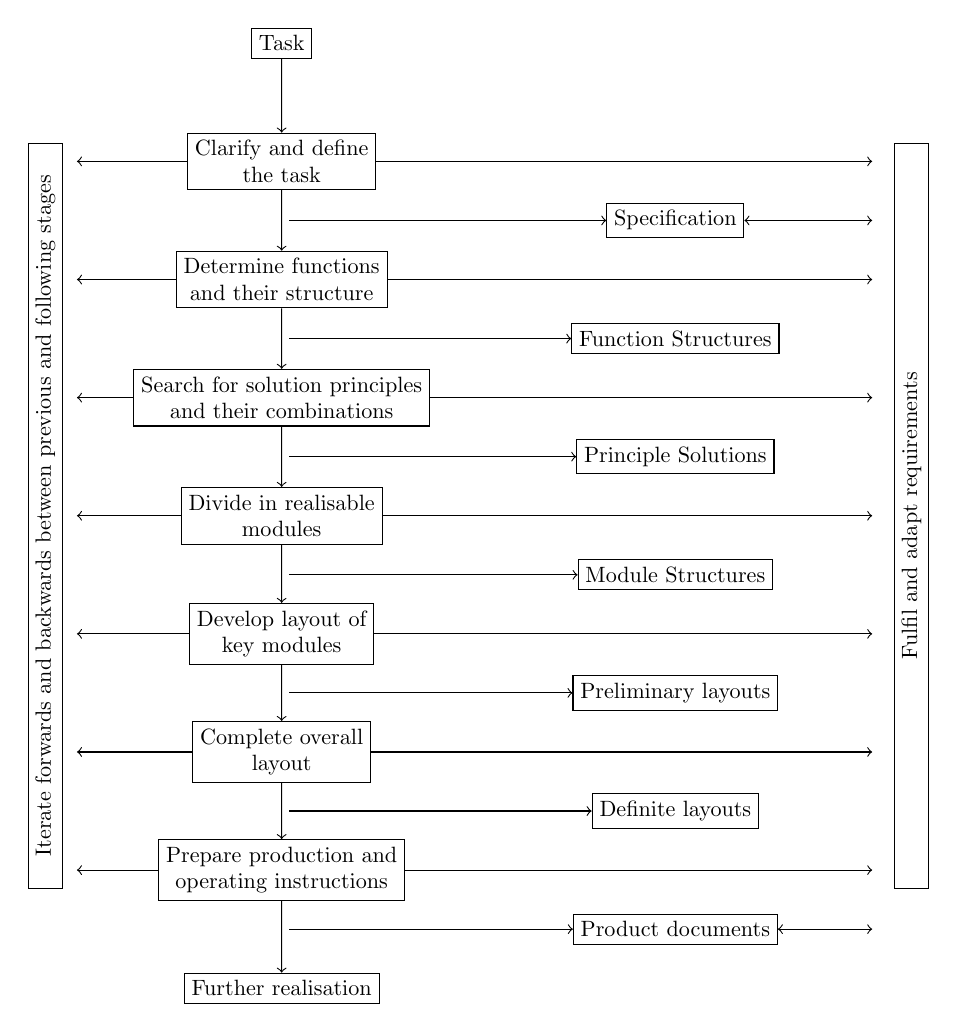
\begin{tikzpicture}[scale=1.0, every node/.style={scale=0.8}]
  \node[align=center, draw] (A) at (0,0) {Task};
  \node[align=center, draw] (B) at (0,-1.5) {Clarify and define\\ the task};
  \draw[->] (A) -- (B);
  \node[align=center, draw] (C) at (0,-3) {Determine functions\\ and their structure};
  \draw[->] (B) -- (C);
  \node[align=center, draw] (D) at (0,-4.5) {Search for solution principles\\ and their combinations};
  \draw[->] (C) -- (D);
  \node[align=center, draw] (E) at (0,-6) {Divide in realisable\\ modules};
  \draw[->] (D) -- (E);
  \node[align=center, draw] (F) at (0,-7.5) {Develop layout of\\ key modules};]
  \draw[->] (E) -- (F);
  \node[align=center, draw] (G) at (0,-9) {Complete overall\\ layout};
  \draw[->] (F) -- (G);
  \node[align=center, draw] (H) at (0,-10.5) {Prepare production and\\ operating instructions};
  \draw[->] (G) -- (H);
  \node[align=center, draw] (I) at (0,-12) {Further realisation};
  \draw[->] (H) -- (I);

  \node[] (AB) at (0,-2.25) {};
  \node[align=center, draw] (J) at (5,-2.25) {Specification};
  \draw[->] (AB) -- (J);

  \node[] (BC) at (0,-3.75) {};
  \node[align=center, draw] (K) at (5,-3.75) {Function Structures};
  \draw[->] (BC) -- (K);

  \node[] (CD) at (0,-5.25) {};
  \node[align=center, draw] (L) at (5,-5.25) {Principle Solutions};
  \draw[->] (CD) -- (L);

  \node[] (DE) at (0,-6.75) {};
  \node[align=center, draw] (M) at (5,-6.75) {Module Structures};
  \draw[->] (DE) -- (M);

  \node[] (EF) at (0,-8.25) {};
  \node[align=center, draw] (N) at (5,-8.25) {Preliminary layouts};
  \draw[->] (EF) -- (N);

  \node[] (FG) at (0,-9.75) {};
  \node[align=center, draw] (O) at (5,-9.75) {Definite layouts};
  \draw[->] (FG) -- (O);

  \node[] (GH) at (0,-11.25) {};
  \node[align=center, draw] (P) at (5,-11.25) {Product documents};
  \draw[->] (GH) -- (P);

  \node[align=center, draw, rotate=90, text width=330] (Q) at (-3,-6) {Iterate forwards and backwards between previous and following stages};
  \draw[->] (B) -- (-2.6,-1.5);
  \draw[->] (C) -- (-2.6,-3);
  \draw[->] (D) -- (-2.6,-4.5);
  \draw[->] (E) -- (-2.6,-6);
  \draw[->] (F) -- (-2.6,-7.5);
  \draw[->] (G) -- (-2.6,-9);
  \draw[->] (H) -- (-2.6,-10.5);

  \node[align=center, draw, rotate=90, text width=330] (Q) at (8,-6) {Fulfil and adapt requirements};
  \draw[->] (B) -- (7.5,-1.5);
  \draw[->] (C) -- (7.5,-3);
  \draw[->] (D) -- (7.5,-4.5);
  \draw[->] (E) -- (7.5,-6);
  \draw[->] (F) -- (7.5,-7.5);
  \draw[->] (G) -- (7.5,-9);
  \draw[->] (H) -- (7.5,-10.5);

  \draw[<->] (P) -- (7.5,-11.25);
  \draw[<->] (J) -- (7.5,-2.25);

\end{tikzpicture}
  }
  \caption[Systematic design approach]{Systematic design approach~\citep{pahl2013}}\label{fig-vdi}
\end{figure}

Some of the activities that you will be doing in this exercise are as follows:

\begin{enumerate}
  \item Product Design Specification
  \item Initial Calculations
  \item Arrangement Selection
  \item Initial Shaft Sizing
  \item Transmission Selection
  \item Bearing Selection
  \item Fixtures \& Fittings
  \item Engineering Drawing
\end{enumerate}

It is important to note that the order in which you perform these activities and where you do your iterations may be different to your peers. As a engineering designer, you will need to clearly articulate the process you have gone through to complete the exercise.

The rest of this document contains content that is pertinent to the activities you will be performing to develop a component capable of surviving the forces that it will be subjected to. Elements have also been left blank where it is expected that you perform some of your own research, attend the lectures \& tutorials to support your design work.
